In Section~\ref{sec:experiments}, we demonstrate the generalization performance of LP-RFFs on the TIMIT and YearPred datasets. In this section, we demonstrate the full generalization performance comparison on the TIMIT, YearPred, CovType and Census datasets. In Figure~\ref{fig:generalization_col_app}, we show the generalization performance of 8, 4, 1 bit LP-RFFs, with FP-\Nystrom, FP-RFF and circulant FP-RFF as the full precision baselines. We can observe that LP-RFF, by using 4 or 8 bit quantized representation, can systematically outperform full precision baselines across the four datasets under different memory budgets.
\begin{figure}
	\centering
	\begin{tabular}{@{\hskip 0in}c@{\hskip 0in}c@{\hskip 0in}c@{\hskip 0in}c@{\hskip 0in}}
%		\subfigure[Census heldout MSE]{\label{fig:census_mem} 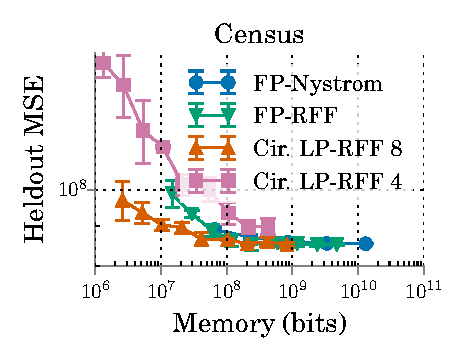
\includegraphics[width=0.3\linewidth]{figures/census_MSE_vs_n_memory.pdf} } \hfill
%		\subfigure[Census heldout MSE]{\label{fig:census_feat}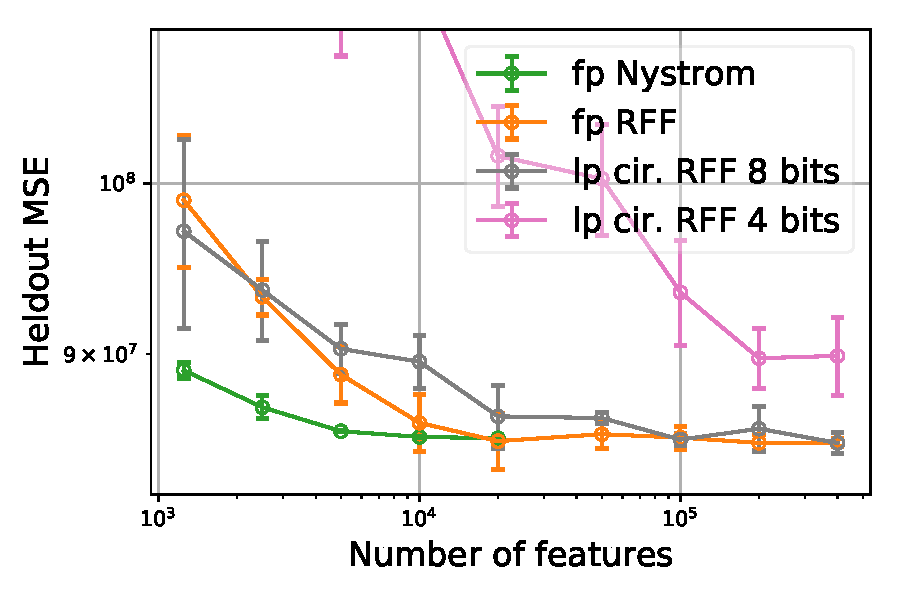
\includegraphics[width=0.3\linewidth]{figures/census_MSE_vs_n_feat.pdf} } \hfill
%		\subfigure[CovType heldout error]{\label{fig:covtype_mem} 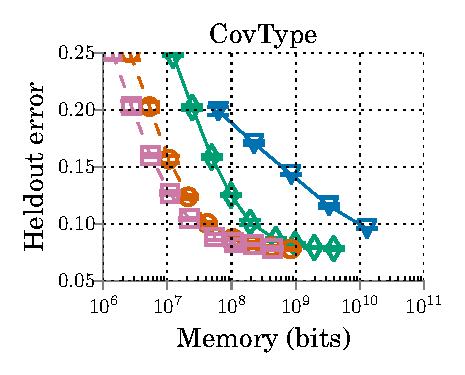
\includegraphics[width=0.3\linewidth]{figures/covtype_error_vs_n_memory.pdf} } \hfill
%		\subfigure[CovType heldout error]{\label{fig:covtype_feat}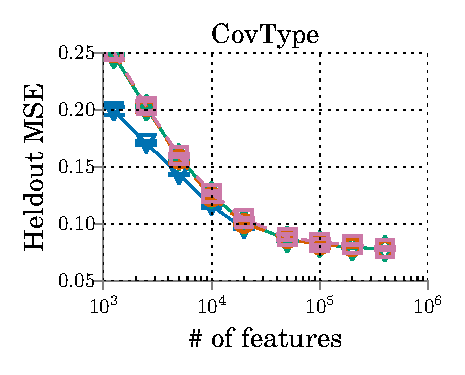
\includegraphics[width=0.3\linewidth]{figures/covtype_error_vs_n_feat.pdf} } \hfill
%		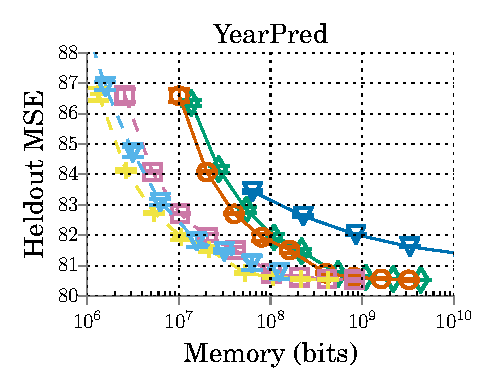
\includegraphics[width=0.3\linewidth]{figures/yearpred_MSE_vs_n_memory_all_line.pdf} &
%		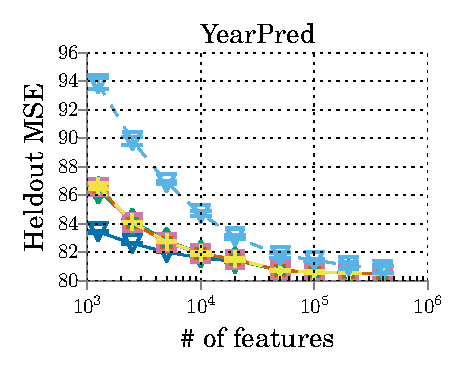
\includegraphics[width=0.3\linewidth]{figures/yearpred_MSE_vs_n_feat_all_line.pdf} &
%		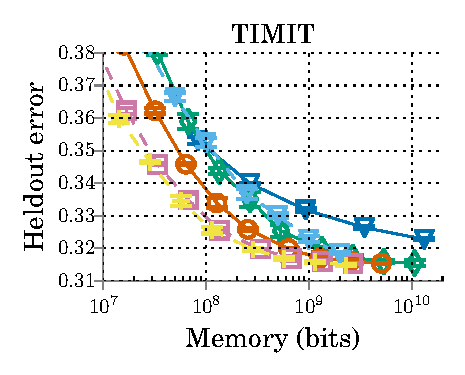
\includegraphics[width=0.3\linewidth]{figures/timit_error_vs_n_memory_all_line.pdf} &
%		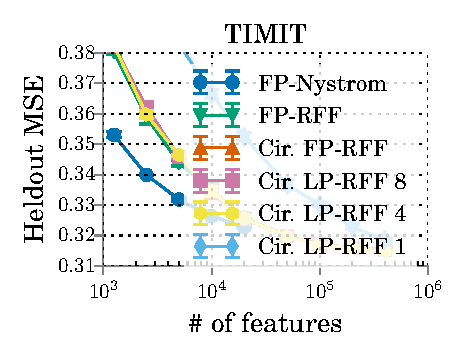
\includegraphics[width=0.3\linewidth]{figures/timit_error_vs_n_feat_all_line.pdf} \\
%		(a) Census & (b) YearPred & (c) Covtype & (d) TIMIT \\
		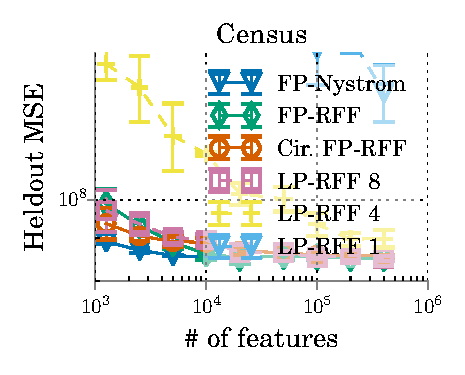
\includegraphics[width=0.26\linewidth]{figures/census_MSE_vs_n_feat_all_line.pdf} &
		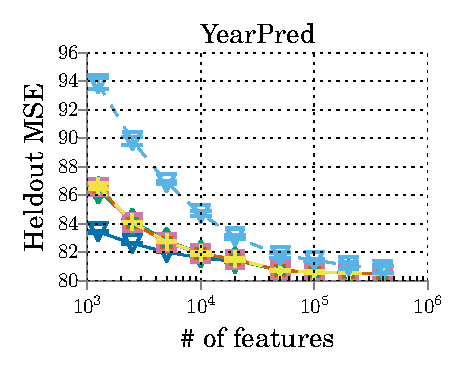
\includegraphics[width=0.26\linewidth]{figures/yearpred_MSE_vs_n_feat_all_line.pdf} &
		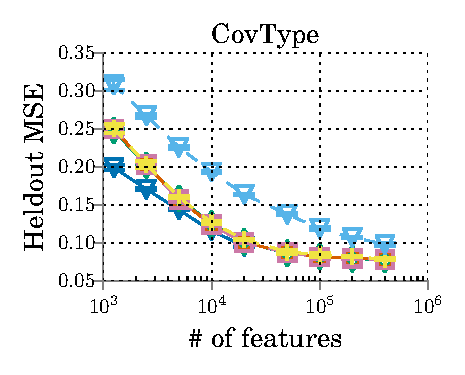
\includegraphics[width=0.26\linewidth]{figures/covtype_error_vs_n_feat_all_line.pdf} &
		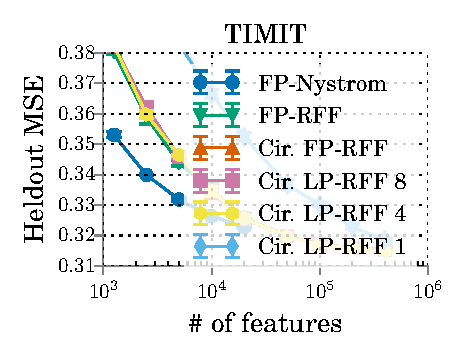
\includegraphics[width=0.26\linewidth]{figures/timit_error_vs_n_feat_all_line.pdf} \\
		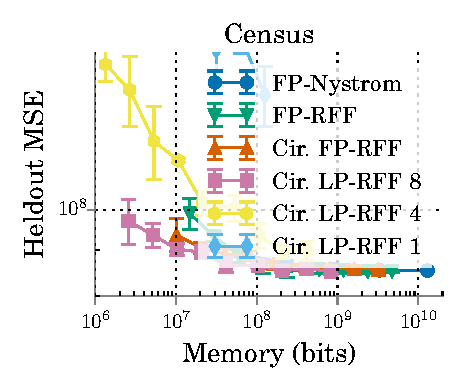
\includegraphics[width=0.26\linewidth]{figures/census_MSE_vs_n_memory_all_line.pdf} &
		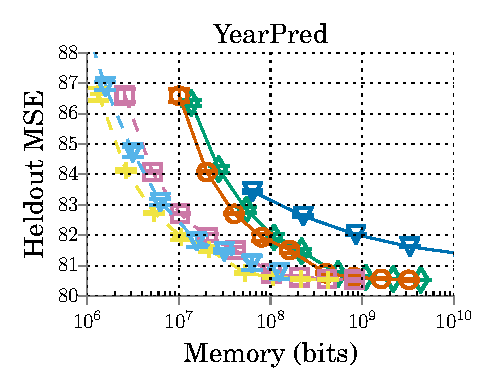
\includegraphics[width=0.26\linewidth]{figures/yearpred_MSE_vs_n_memory_all_line.pdf} &
		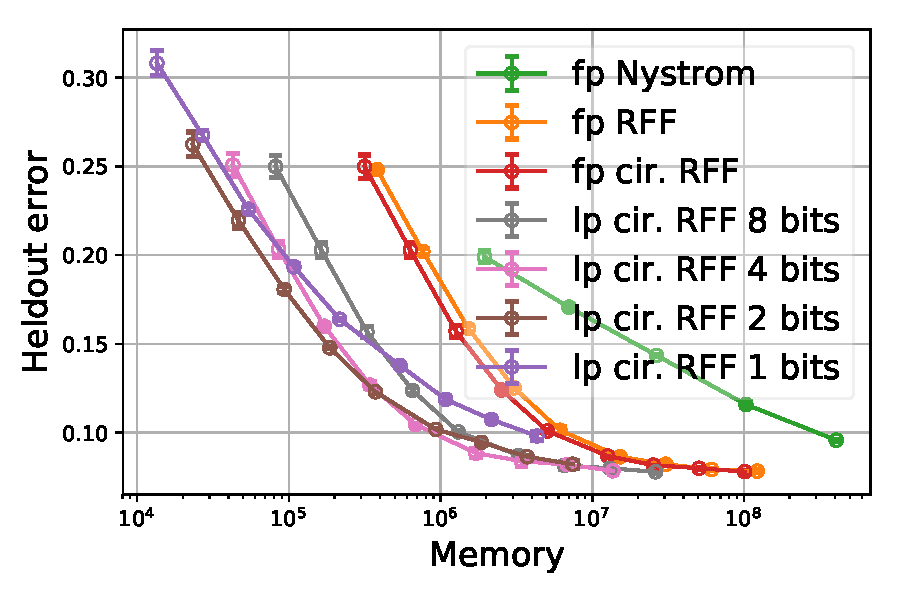
\includegraphics[width=0.26\linewidth]{figures/covtype_error_vs_n_memory_all_line.pdf} &
		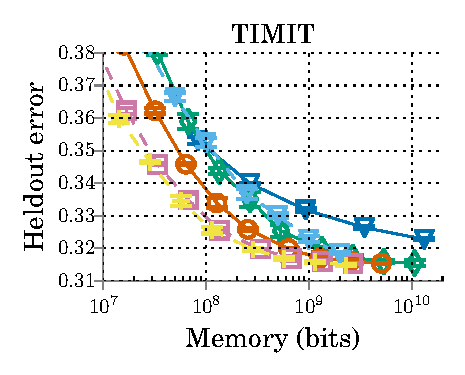
\includegraphics[width=0.26\linewidth]{figures/timit_error_vs_n_memory_all_line.pdf} \\
%		(a) Census & (b) YearPred & (c) Covtype & (d) TIMIT \\
	\end{tabular}
	\caption{Generalization performance of LP RFF, full precision RFF and \Nystrom with respect to number of features and memory budgets. We can observe that LP RFFs demonstrate better generalization performance than full precision baselines under memory budget. Noticeably, the comparison of different methods on generalization performance behaves differently under memory budget and under number off features. E.g., \Nystrom shows better generalization performance than RFF based approach with the same number of features. However, \Nystrom can be significantly worse under memory budgets.}
	\label{fig:generalization_col_app}
\end{figure}

\begin{figure}
	\centering
	\begin{tabular}{@{\hskip -0.25in}c@{\hskip -0.25in}c@{\hskip -0.25in}c@{\hskip -0.25in}}
		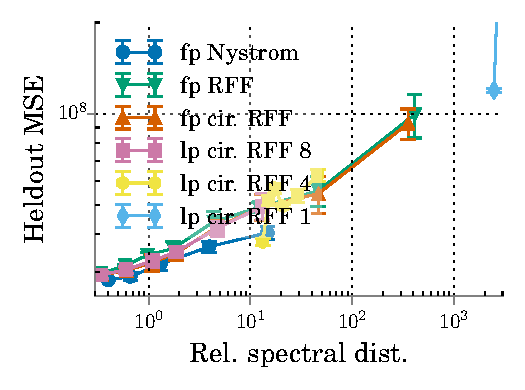
\includegraphics[width=0.33\linewidth]{figures/regression_l2_vs_delta_all_line.pdf} &
		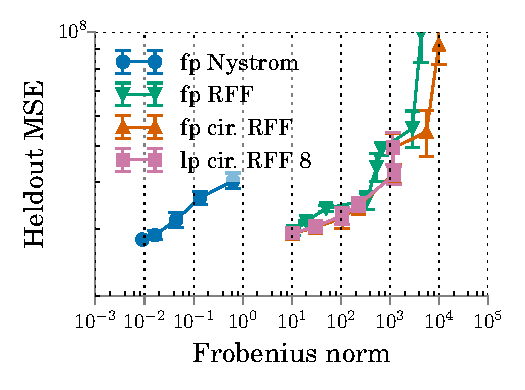
\includegraphics[width=0.33\linewidth]{figures/regression_l2_vs_f_norm_all_line.pdf} &
		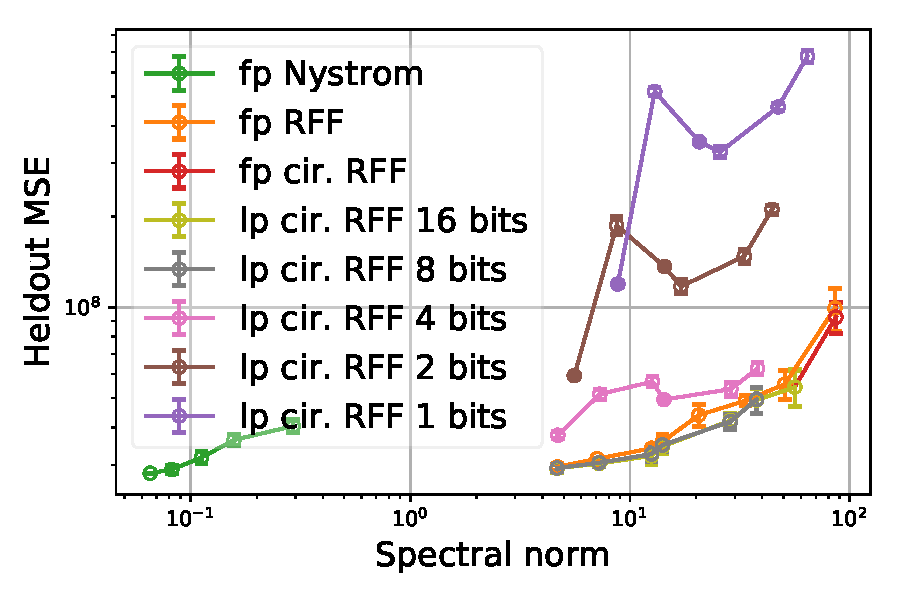
\includegraphics[width=0.33\linewidth]{figures/regression_l2_vs_s_norm_all_line.pdf} \\
		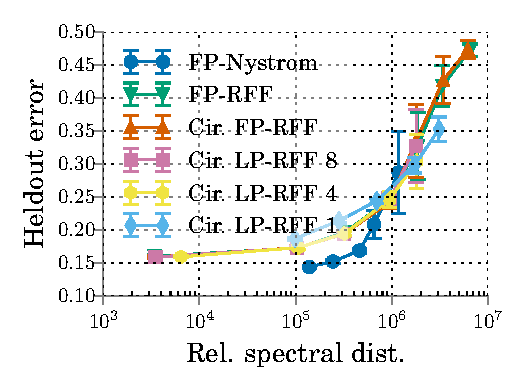
\includegraphics[width=0.33\linewidth]{figures/classification_acc_vs_delta_all_line.pdf} &
		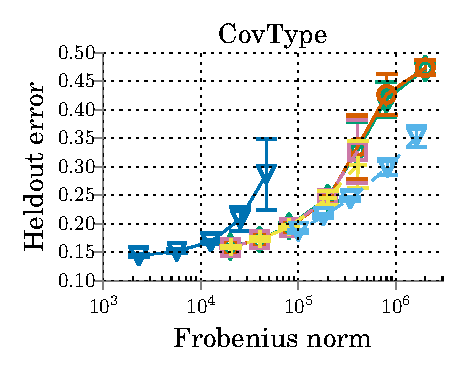
\includegraphics[width=0.33\linewidth]{figures/classification_acc_vs_f_norm_all_line.pdf} &
		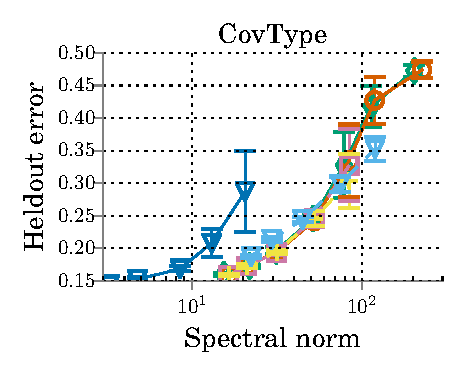
\includegraphics[width=0.33\linewidth]{figures/classification_acc_vs_s_norm_all_line.pdf} \\
	\end{tabular}
%	\begin{tabular}{@{\hskip -0.25in}c@{\hskip -0.25in}c@{\hskip -0.25in}c@{\hskip -0.25in}}
%		\subfigure[MSE and Rel. spectral distance distance]{\label{fig:census_delta_all_line} 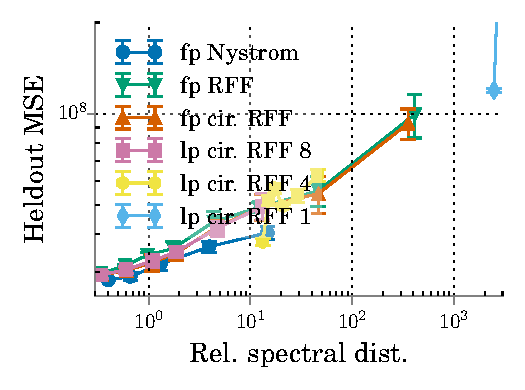
\includegraphics[width=0.33\linewidth]{figures/regression_l2_vs_delta_all_line.pdf} } \hfill
%		\subfigure[MSE and Frobenius norm]{\label{fig:census_f_norm_all_line} 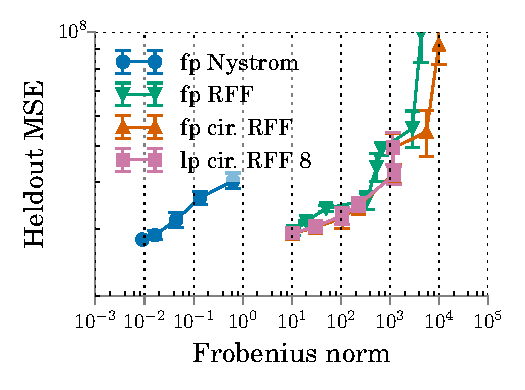
\includegraphics[width=0.33\linewidth]{figures/regression_l2_vs_f_norm_all_line.pdf} } \hfill
%		\subfigure[Rel. spectral distance distance and memory]{\label{fig:census_s_norm_all_line}  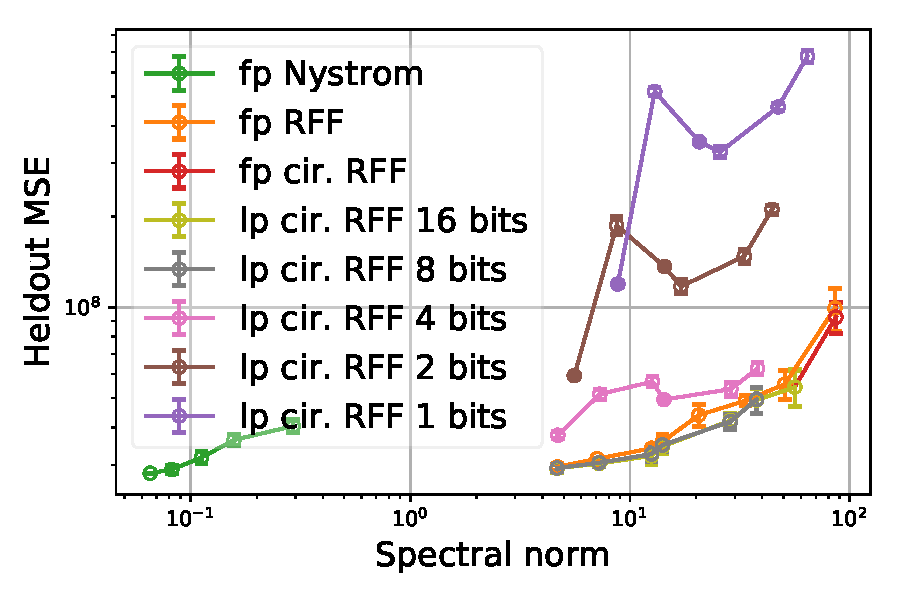
\includegraphics[width=0.33\linewidth]{figures/regression_l2_vs_s_norm_all_line.pdf} } \hfill \\
%		\subfigure[MSE and Frobenius norm]{\label{fig:covtype_delta_all_line} 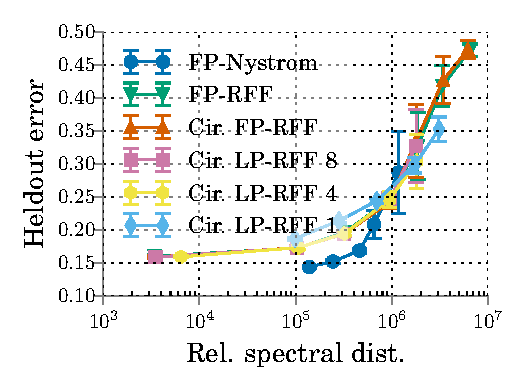
\includegraphics[width=0.33\linewidth]{figures/classification_acc_vs_delta_all_line.pdf} } \hfill
%		\subfigure[Error and Frobenius norm]{\label{fig:covtype_f_norm_all_line} 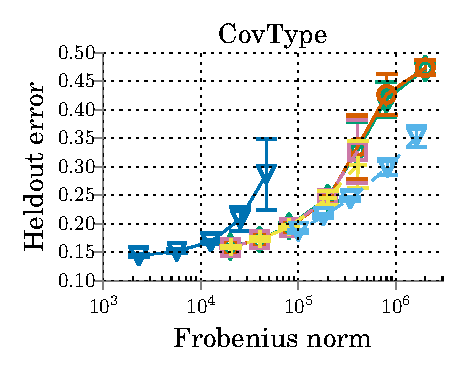
\includegraphics[width=0.33\linewidth]{figures/classification_acc_vs_f_norm_all_line.pdf} } \hfill
%		\subfigure[Error and spectral norm]{\label{fig:covtype_s_norm_all_line} 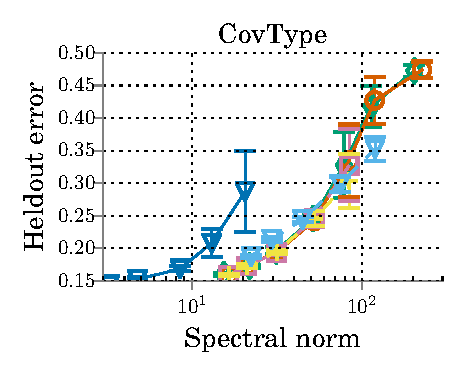
\includegraphics[width=0.33\linewidth]{figures/classification_acc_vs_s_norm_all_line.pdf}} \hfill
%	\end{tabular}
	\caption{Generalization performance vs. relative spectral distance $D_{\lambda}(K,\tK)$, and that Frobenius and spectral norms of $K - \tK$. We observe that $D_{\lambda}(K,\tK)$ aligns much better with generalization performance than the Frobenius and spectral norms, for both the Census and sub-sampled CovType datasets.}
	\label{fig:specdist_app}	
%	\begin{tabular}{c c c}
%		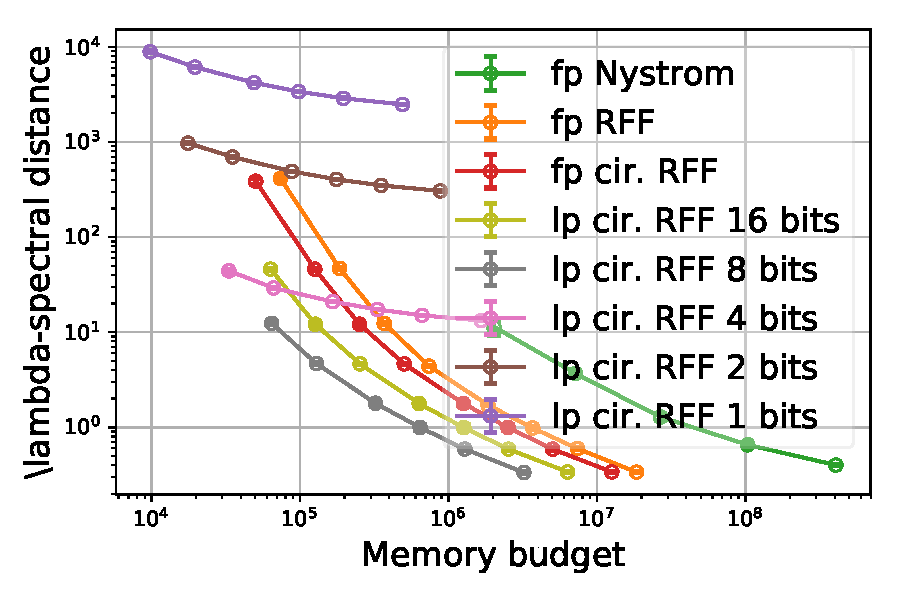
\includegraphics[width=0.33\linewidth]{figures/regression_delta_vs_mem_all_line.pdf} &
%		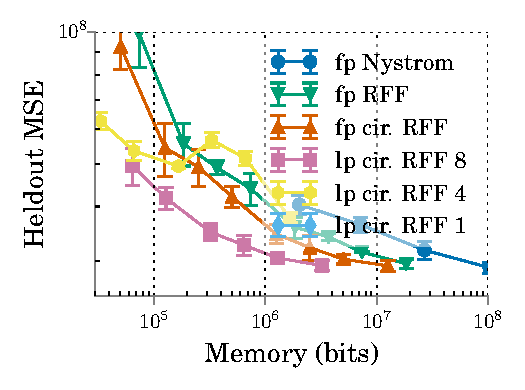
\includegraphics[width=0.33\linewidth]{figures/regression_l2_vs_mem_all_line.pdf} &
%		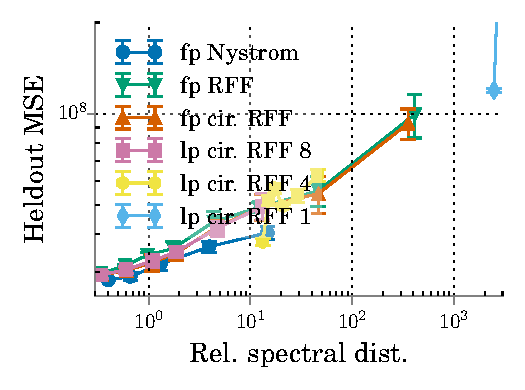
\includegraphics[width=0.33\linewidth]{figures/regression_l2_vs_delta_all_line.pdf} \\
%		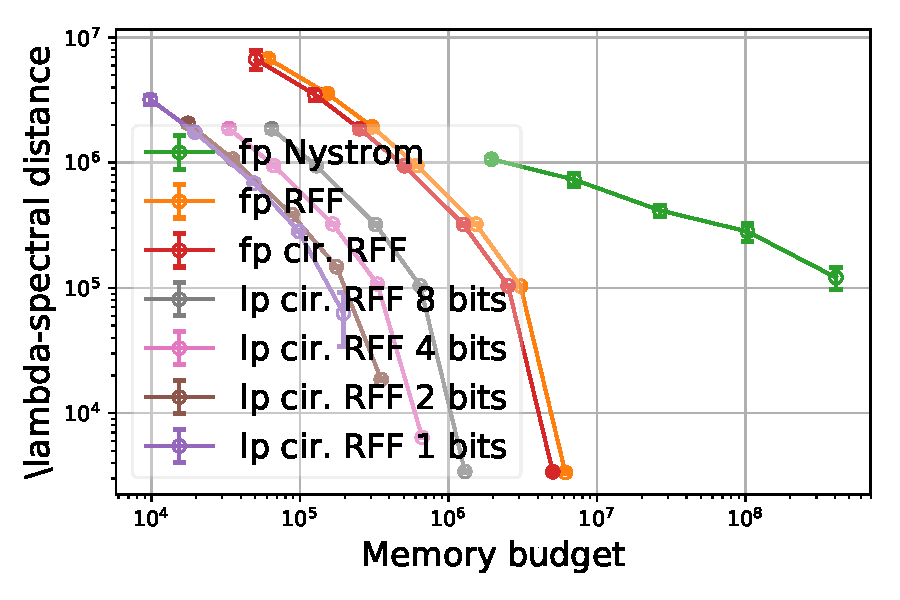
\includegraphics[width=0.33\linewidth]{figures/classification_delta_vs_mem_all_line.pdf} &
%		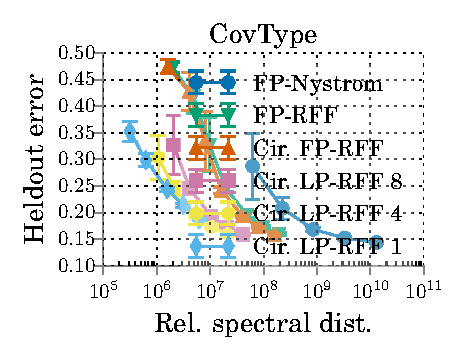
\includegraphics[width=0.33\linewidth]{figures/classification_acc_vs_mem_all_line.pdf} &
%		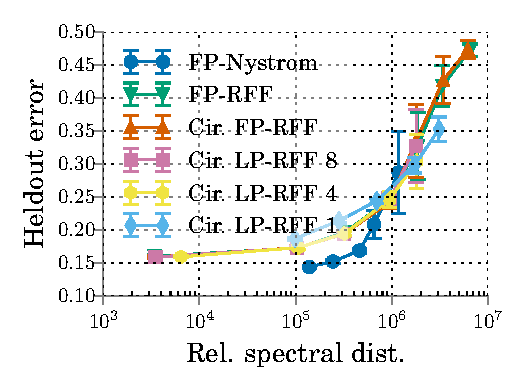
\includegraphics[width=0.33\linewidth]{figures/classification_acc_vs_delta_all_line.pdf} \\
%		(a) & (b) & (c)
%	\end{tabular}
%	\caption{The strong correlation between generalization performance and $\lambda$-spectral distance $D_{\lambda}(K,\tK)$ under memory budgets for the Census dataset (top) and subsampled CovType dataset (bottom). Under different memory budget in (a) and (b), the precision demonstrates smaller $D_{\lambda}(K,\tK)$ tends to have better generalization performance. In (c), different kernel approximation approaches demonstrate similar generalization performance for similar $\lambda$-spectral distance.}
%	\label{fig:specdist_app}
\end{figure}

